\input{R1_template}

\begin{document}

\title{Basic relic density calculator}
%
\author
{
  James McKay\thanksref{e1,addr1}
}
%
\thankstext{e1}{e-mail: j.mckay14@imperial.ac.uk}
%
\institute
{
  Imperial College London\label{addr1}
}
%
\date{\today}

\maketitle

\begin{abstract}
This program is designed to quickly calculate the relic density of a weakly interacting massive particle (WIMP) by solving the Boltzman equation via a user specified method.  We focus primarily on the case of a simple scalar singlet extensions to the standard model including semi-annihilation processes, however a range of possible WIMP models may be implemented in this program due to the generic nature of the core functions.
\end{abstract}

\tableofcontents

\section{Introduction}

The dark matter relic density is the mass which is required to fill deficit predicted by the standard $\Lambda$CDM cosmology.  This mass density, substantially greater than the density of standard model (SM) particles, must be filled by a slow moving weakly interacting particle massive particle (WIMP).  The value of the relic density was set in the early universe, when the temperature was high enough that these WIMP particles were in thermal equilibrium with the standard model particles in the relativistic plasma.  Thus, there was sufficient energy to produce a large quantity of WIIMP particles.

Freeze-out occurred when the temperature of the universe dropped sufficiently that the WIMP particles were no longer in equilibrium, and are thus no more dark matter was produced.  The WIMP particles must have at least one stable state.  This is generally imposed by giving the new particles a symmetry, such that the lowest energy particle cannot decay.  Thus production of SM particles from dark matter may only occur through dark matter annihilation or semi-annihilation processes (which, as the universe continues to expand are rare events), thus the density of dark matter is \textit{frozen out}.



\subsection{Solving the Boltzman equation}

We follow the semi-analytic approximation described by Cline et al. \cite{Cline2013} and Steigman et al. \cite{Steigman2012} as a means of quickly obtaining the relic density.

The equation which governs the competition between production and annihilation is
\begin{align}
\frac{dn}{dt}+3Hn=\frac{d(na^3)}{a^3dt}=<\!\sigma v\! >(n_{eq}^2-n^2)\label{eqn:boltz}
\end{align}
where $n$ is the number density of dark matter particles and $a$ is the cosmological scale factor.  By invoking the conservation of entropy (in the absence of phase transitions) in a comoving volume we have that $S\equiv sa^3=(2\pi^2/45)g_sT^3a^3$ is conserved.  So (\ref{eqn:boltz}) can be written in terms of $Y=n/s$ and $Y_{eq}=n_{eq}/s$ where
\begin{align}
Y_{eq}=\frac{n_{eq}}{s}=\frac{45}{2\pi^4}\left(\frac{\pi}{8}\right)^{1/2}\frac{g_{\chi}}{g_s}x^{3/2}\exp(-x)
\end{align}

thus (\ref{eqn:boltz}) becomes
\begin{align}
\frac{dY}{dx}=\left(Y_{eq}^2-Y^2\right)
\end{align}
where
\begin{align}
Z(x)=\sqrt{\frac{\pi}{45}} \frac{M_sM_{Pl}}{x^2} \sqrt{g_{*}}<\!\sigma v\! >
\end{align}

\section{The program structure}

The program is separated into classes, some of which are templated for easy adaptability and inclusion of new models.  

\subsection{The data structure}
Essential for almost all classes is the \lstinline{Data} structure, which holds the default SM parameters and physical constants, and reads in an input file.  The input file is passed at run time via \lstinline{./main input.txt} where \lstinline{input.txt} is a data file in the form

\begin{lstterm}
M_s         800
lambda_hs   0.1
M_h         126
M_w         91
\end{lstterm}

where the user has defined the scalar singlet mass to be 800 GeV, the coupling $\lambda_{hs}$ to be 0.1 and reset the SM masses for the Higgs and W boson to non-standard values.  The full list of parameters that are available to be reset via the input file, and the correct name to use, are given in table X.  If no input file is provided at run time, the most recent experimental values will be chosen for all parameters including unknown beyond SM parameters, which are given arbitrary values for the sake of example.

\subsection{The relic density class}

The central class for performing the calculations is \lstinline{Relic_density<Model_name>}, which takes a model typename as template parameter and a \lstinline{Data} structure as an argument.  This class calls on further functions defined in \lstinline{integrate.hpp}, \lstinline{interp.hpp} and \lstinline{bessel.hpp} to perform integrals, interpolations and calculating bessel functions.  The bessel function class will return either an asymptotic approximations for large values of the arguments, or use the standard Boost library when the approximation is not appropriate.


The function \lstinline{calc_cross_section} will perform the thermal average \cite{Cline2013}
\begin{align}
<\!\!\sigma v_{rel}\!\!>=\int_{4m_s^2}^{\infty}\frac{s\sqrt{s-4m_s^2}K_1(\sqrt{s}/T)\sigma v_{rel}} { 16 T m_s^4K_2^2(m_s/T)} \label{thermal_av}
\end{align}
where $\sigma v_{rel}$ is provided by the model class, which must have a member function \lstinline{cs_integral}.  For the case of the scalar singlet model this is
\begin{align}
\sigma v_{rel}=\frac{2\lambda_{hs}^2v_0^2}{\sqrt{s}} |D_h(s)|^2\Gamma_h(\sqrt{s}) \label{eqn:sv}
\end{align}
where 
\begin{align}
 |D_h(s)|^2\equiv \frac{1}{ (s-M_h^2)^2+M_h^2\Gamma_h^2(m_h)}
 \end{align}
\begin{figure}
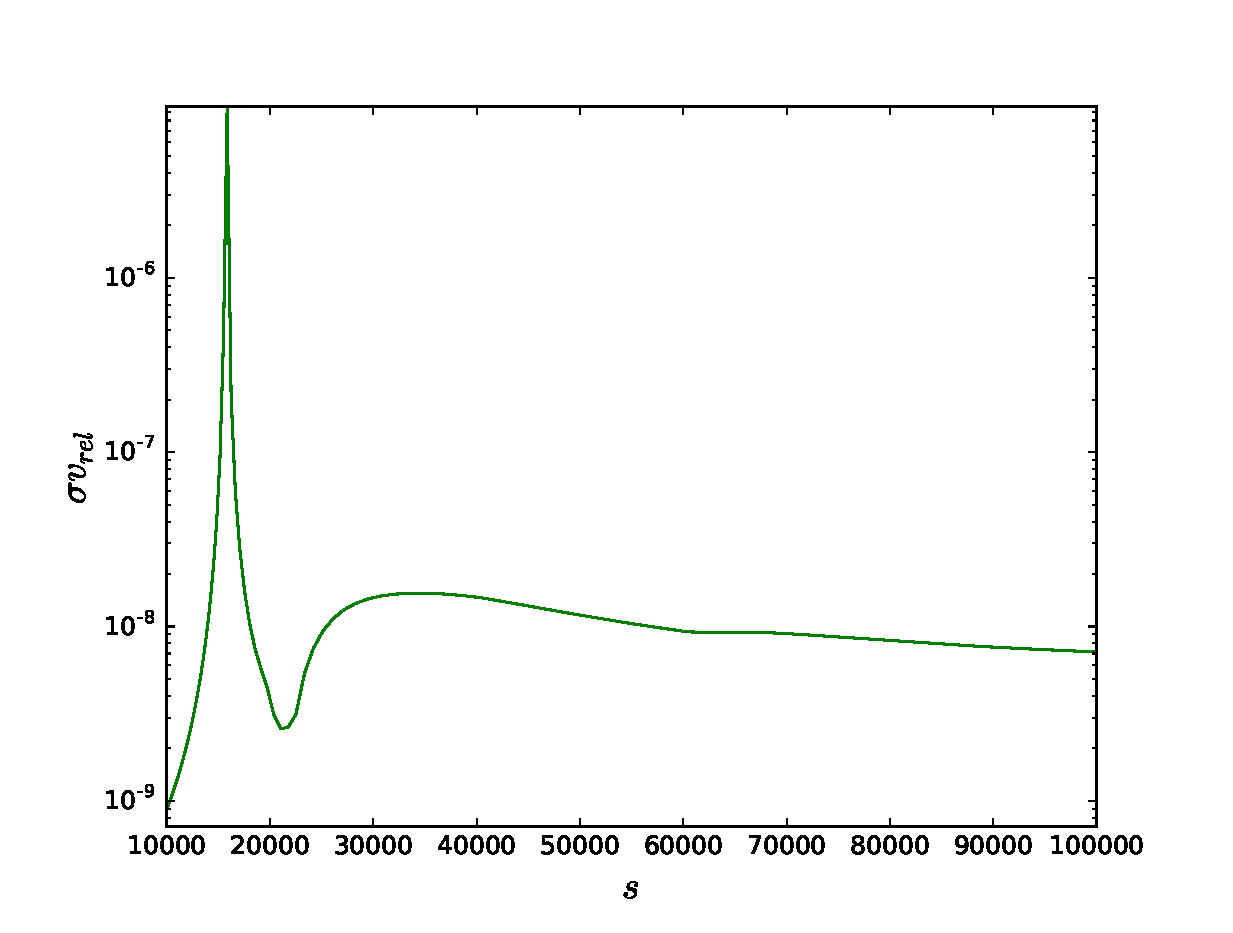
\includegraphics[width=0.5\textwidth]{resonance.eps}
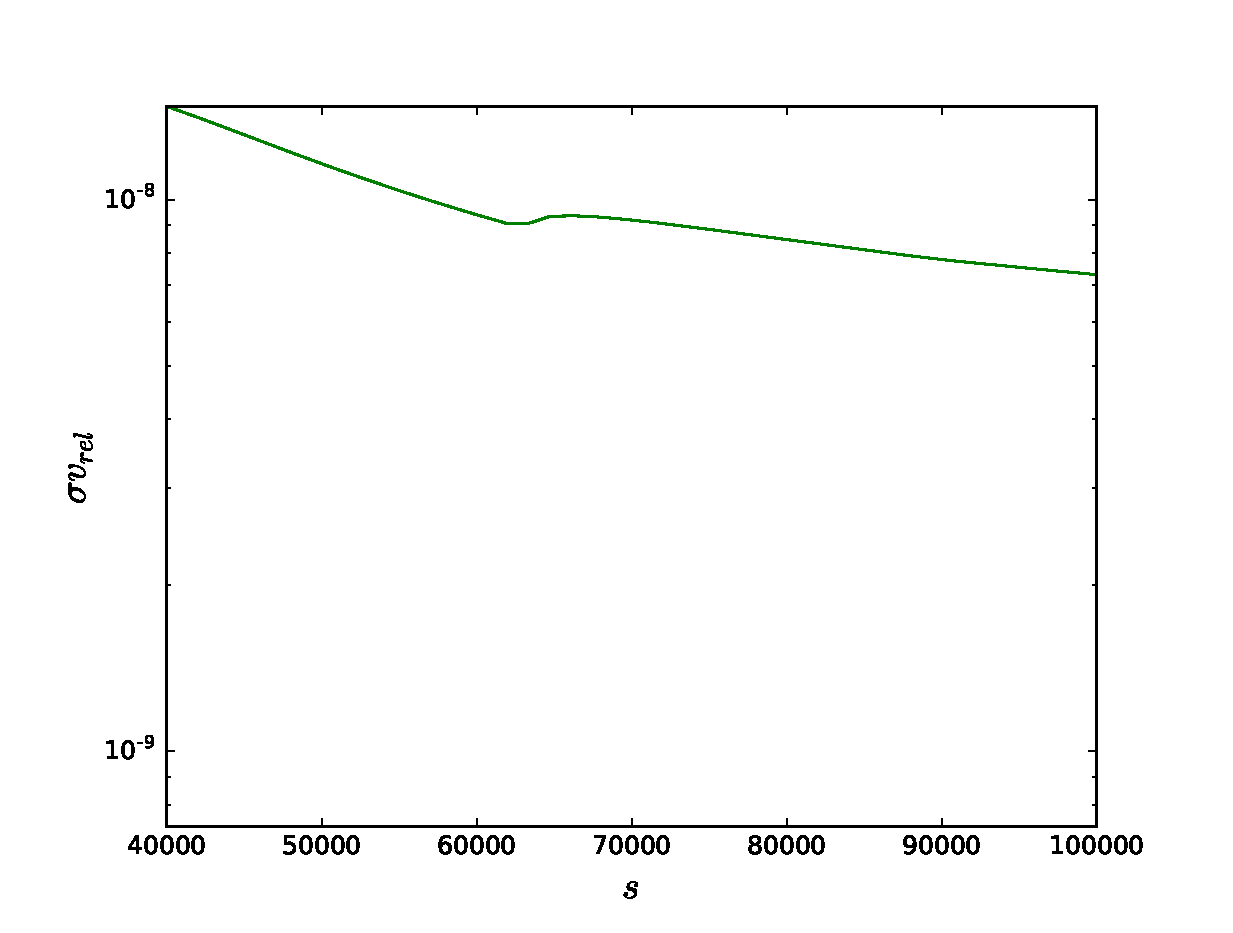
\includegraphics[width=0.5\textwidth]{no_resonance.eps}
\caption{$\sigma v$, (\ref{eqn:sv}), as a function of $s$ for $m_s=50$ GeV (left) and $m_s=100$ GeV (right), where on the left we see a resonance at $s=m_h^2/4$ as expected.  Note that the vertical scale is very different on these two plots, and the far left point is $s=4m_s^2$ in each case.}\label{fig:Higgs_res}
\end{figure}

We plot (\ref{eqn:sv}) for a scalar mass $m_s=50$ GeV and $m_s=100$ GeV in Figure \ref{fig:Higgs_res}.  This demonstrates the resonance at $4M_s^2\approx M_h$, which is only present for scalar masses sufficiently smaller than the Higgs mass.

The freeze out temperature $x*=m/T*$ is calculated by the function \lstinline{Relic_density<Model>::x_f()} which will return a \lstinline{double} for $x*$.  This will call the structure \lstinline{Z_func<Model>}, which will return $Z(x)$.  This structure takes the model type as a template parameter, and the \lstinline{Data} structure.  When called to calculate $x_f$, since only a few evaluations are required, this will calculate $Z(x)$ from the thermal average each time.

The integral $A(x)$ uses the thermal average (\ref{thermal_av}) via the function \lstinline{Z_func<Model>} extensively during the calculation.  Therefore, it is desirable to tabulate values for $Z(x)$ over the required range and call an interpolation on these values instead.  This is achieved with the member function \lstinline{thermal_average_make_interp}, which is called from \lstinline{Relic_density<Model>::A(double x_f)}.  This fills two arrays, which are then passed as additional arguments to  \lstinline{Z_func<Model>}, which when passed sets this structure to interpolate on the given arrays rather than computing the thermal average at each step. This dramatically increases the speed of the integration.

Finally, the value of $Y$ at the present time is calculated using \lstinline{Relic_density<Model>::Y_today(double x_f)}.  The whole calculation process is simply achieved using the following lines
\begin{lstcpp}
Relic_density<SingletDM_RD> relic_density(data);
double x_f = relic_density.x_f();
double Y = relic_density.Y_today( x_f );
double rho_crit = 1.05375e-5, s_0 = 2890;
return  Y*data.M_s*s_0/rho_crit;
\end{lstcpp}
which will return the dark matter mass fraction $\Omega_{\chi} h^2$ at the present time.  In the above example \lstinline{SinlgetDM_RD} is the model typename, replacing this with another valid name is all that is required to perform calculations in a different model.



\subsection{Model classes}

The model classes are defined in the header \lstinline{model.hpp}, which is the location new model definitions must be added to.  The model definition must be of the form
\begin{lstcpp}
class MODEL_NAME
{
  private:
  Data data;
  public:
  MODEL_NAME_RD (){}  // default constructor
  MODEL_NAME_RD(Data _data)
  {
    data=_data;
   } //constructor
  
  double cs_integral(double s, double T);

  double sigma_v(double s);
 
  Data set_dm_mass(Data data){data.M_dm=data.M_s;return data;};
  
  
};
\end{lstcpp}

The function \lstinline{set_dm_mass} is essential as the generic relic density functions use a generic dark matter mass (as we assume a single, or at least almost mass degenerate dark matter particle content).  In this case, for a scalar singlet model, the dark matter mass is $M_s$, as defined in the input file and thus this is set to $M_{dm}$.  The other required functions are \lstinline{cs_integral} which returns the correctly normalised argument for the integral (\ref{thermal_av}), which is used by \lstinline{Relic_density} to calculate the thermal average.  The function \lstinline{sigma_v} is not required, but is typically used to calculate $\sigma v$ which is then combined with the appropriate Bessel functions and coefficients in \lstinline{cs_integral}.

The member functions in the above example should be written in a separate source file, \lstinline{<model_name>.cpp} in the source directory, with the file name then added to the line \lstinline{set(SRC_FILES <model_name>.cpp) } in the CMakeLists.txt file located in the base directory.

\subsection{The Boltzman solver}

We offer two alternative methods for solving the Boltzman equation.



\section{Semi-annihilation processes}

In certain models semi-annihilation processes are possible.  In this case two dark matter particles can annihilate into a SM and dark matter particle, rather than only SM particles.  This can effect the relic density in certain parts of the parameter space.  We describe the additional decay processes and how these are added to the program here.

The equation for the number density must be modified to include the contribution from semi-annihilation processes,
\begin{align}
\begin{split}
\frac{dn}{dt}=&-v\sigma^{SS*\rightarrow XX}(n^2-\bar{n}^2)-3Hn\\
&-\frac{1}{2}v\sigma^{SS\rightarrow S*h}(n^2-n\bar{n})
\end{split}
\end{align}
where $X$ is any SM particle.  The semi-annihilation fraction is defined to be
\begin{align}
\alpha=\frac{1}{2}\frac{v\sigma^{SS\rightarrow S*h}}{v\sigma^{SS*\rightarrow XX}+\frac{1}{2}v\sigma^{SS*\rightarrow S*h}}
\end{align}

the freeze-out condition becomes
\begin{align}
x_f=\log \left[ \frac{Z(x) Y_{eq}^2}{Y_{eq}-\frac{d Y_{eq}}{dx}} \frac{\delta (\delta+2-\alpha)}{(1+\delta)}\right]
\end{align}



the resultant equation to solve is
\begin{align}
\frac{dY}{dx}=Z(x)(Y_{eq}^2(1-\alpha)+\alpha Y Y_{eq}-Y^2)
\end{align}





\section{The plotting routines}



\section{Example results}
\begin{figure}
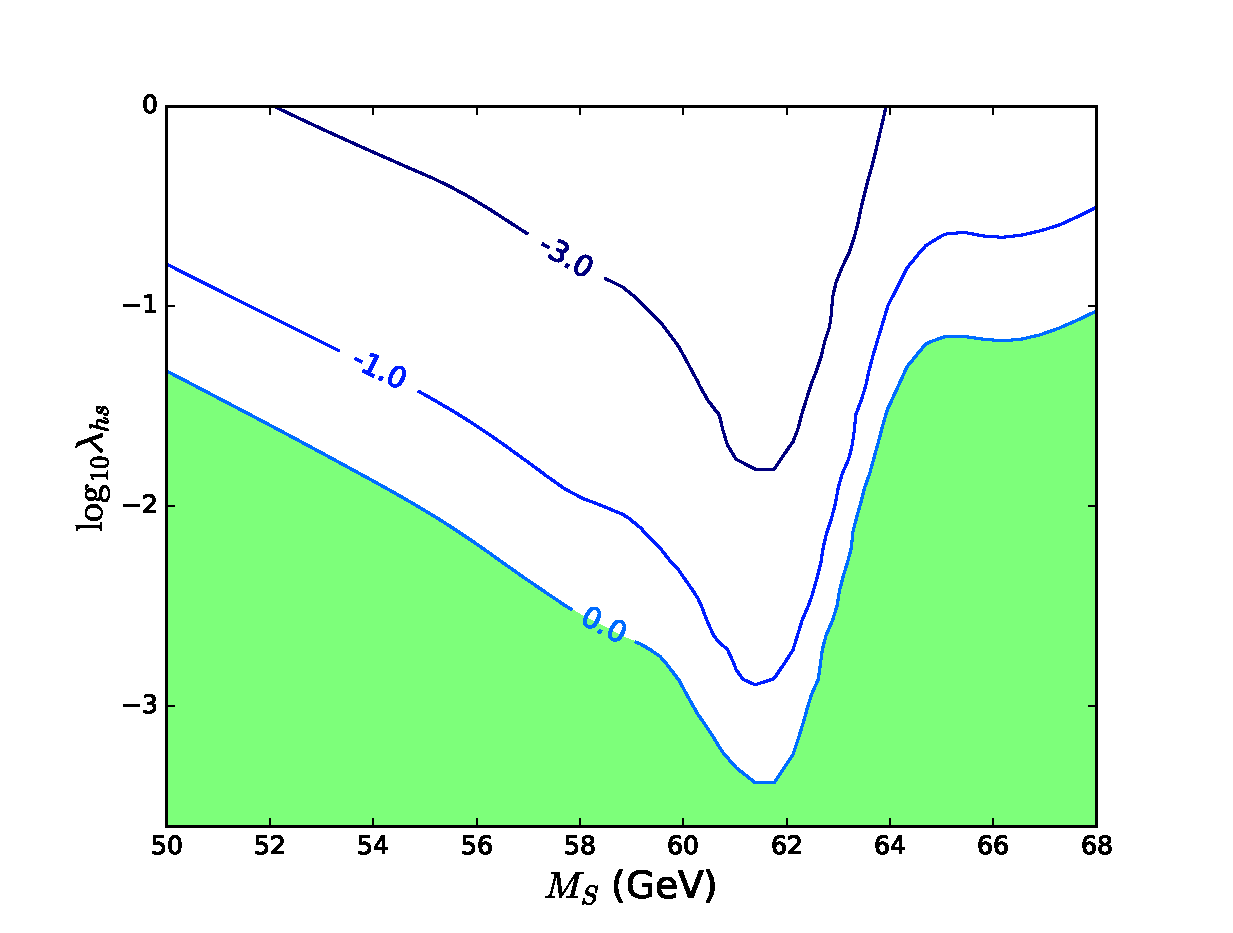
\includegraphics[width=0.5\textwidth]{relic_density.eps}
\caption{The relic density contours for the scalar singlet model.}\label{fig:rd_scan}
\end{figure}





\bibliography{../../../Papers/library}{}


\end{document}  